\documentclass[12pt,a4paper]{article}

\usepackage[utf8]{inputenc}
\usepackage[T1]{fontenc}
\usepackage[english]{babel}
\usepackage{geometry}
\usepackage{enumitem}
\usepackage{amsmath}
\usepackage{hyperref}
\usepackage{microtype}
\usepackage{graphicx}
\usepackage{float}
\usepackage{tikz}
\usetikzlibrary{patterns}

% --- Spacing (compact, professional) ---
\setlength{\parskip}{3pt}
\setlength{\parindent}{0pt}

\setlist[itemize]{itemsep=1pt, topsep=2pt, parsep=0pt, partopsep=0pt}
\setlist[enumerate]{itemsep=1pt, topsep=2pt, parsep=0pt, partopsep=0pt}

\usepackage{titlesec}
\titlespacing*{\section}{0pt}{6pt}{4pt}
\titlespacing*{\subsection}{0pt}{5pt}{3pt}
\titlespacing*{\subsubsection}{0pt}{4pt}{2pt}

\setlength{\textfloatsep}{8pt}
\setlength{\intextsep}{6pt}
\setlength{\floatsep}{6pt}
\geometry{margin=2.0cm}

\hypersetup{
    colorlinks=true,
    linkcolor=black,
    urlcolor=black
}

\title{
\textbf{\Large Benchmark of AI Tools for Industrial Application Development}\\
{\large 2D Palletization (Single-Bin, Python 3.10+, PyQt5)}
}

\author{
Roman Parák, JIC Smart Factory
}

\date{\today
}


\begin{document}

\pagestyle{plain}

\maketitle

%-------------------------------------------------
\section{Purpose of the Benchmark}

The purpose of this benchmark is to objectively compare selected AI tools during the development of a realistic industrial application.

Each team member will implement an application that solves the problem of \textbf{2D palletization (2D bin packing)} on a single pallet, with the goal of using the pallet area efficiently. The application will include an algorithmic core and a graphical user interface built with PyQt5.

The benchmark will be carried out using the following tools:

\begin{itemize}
    \item ChatGPT -- Codex
    \item Cursor
    \item Claude Code
\end{itemize}

The outcome will be a functional application, a documented development process, and a structured evaluation of the AI tool.

%-------------------------------------------------
\subsection{Illustration of the 2D Palletization Problem}

Figure~\ref{fig:binpacking_schema} schematically illustrates the principle
of 2D palletization (single-bin). The rectangle represents a pallet with
dimensions $W \times H$. The smaller rectangles represent individual items.
Items must not overlap and must respect the minimum distance $g$.

\begin{figure}[H]
\centering
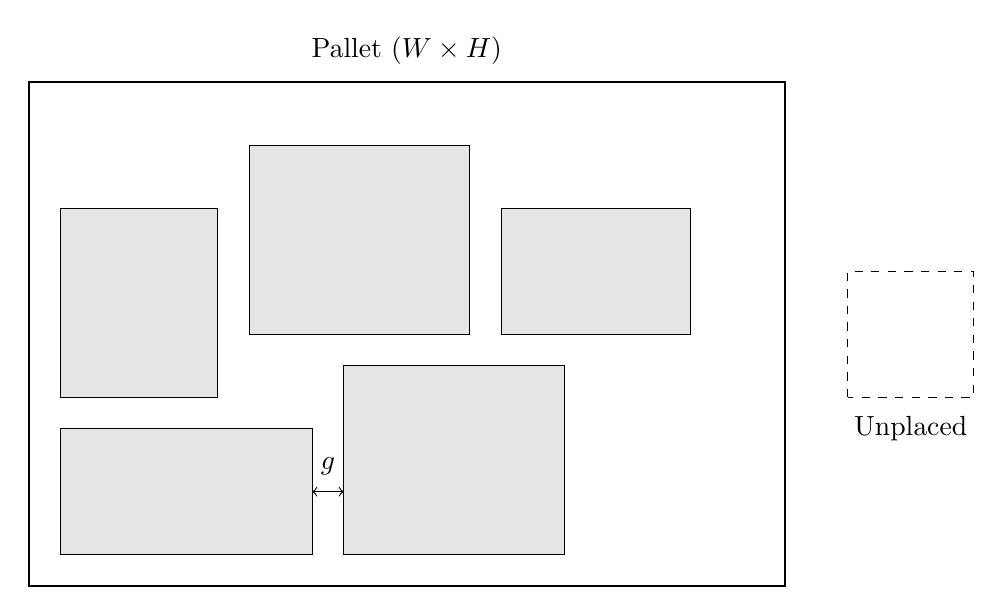
\begin{tikzpicture}[scale=0.8]

% Pallet
\draw[thick] (0,0) rectangle (12,8);
\node at (6,8.5) {Pallet ($W \times H$)};

% Items
\draw[fill=gray!20] (0.5,0.5) rectangle (4.5,2.5);
\draw[fill=gray!20] (5,0.5) rectangle (8.5,3.5);
\draw[fill=gray!20] (0.5,3) rectangle (3,6);
\draw[fill=gray!20] (3.5,4) rectangle (7,7);

% Rotated item
\draw[fill=gray!20] (7.5,4) rectangle (10.5,6);

% Unplaced item (outside the pallet)
\draw[dashed] (13,3) rectangle (15,5);
\node at (14,2.5) {Unplaced};

% Gap g label
\draw[<->] (4.5,1.5) -- (5,1.5);
\node at (4.75,1.9) {$g$};

\end{tikzpicture}
\caption{Schematic illustration of the 2D palletization problem (single-bin).}
\label{fig:binpacking_schema}
\end{figure}

%-------------------------------------------------
\section{Functional Requirements}

\subsection{Purpose and Scope of the Solution}

The task is to implement a solution for 2D palletization on a single pallet (single-bin).

The goal is to:

\begin{itemize}
    \item prevent item overlap,
    \item maintain the minimum gap between items,
    \item ensure that items are placed inside the pallet,
    \item maximize pallet area utilization.
\end{itemize}

The solution may be heuristic. Finding the global optimum is not required.

%-------------------------------------------------
\subsection{Input Parameters}

\textbf{Pallet (Bin)}

\begin{itemize}
    \item $W$ -- pallet width [mm]
    \item $H$ -- pallet height [mm]
    \item $g$ -- minimum gap between two items [mm]
\end{itemize}

Constraints:

\begin{enumerate}
    \item Each item must be placed inside the $W \times H$ area.
    \item The minimum distance between any two items must be at least $g$.
    \item No gap is required between an item and the pallet boundary.
\end{enumerate}

\textbf{Items}

For item types $i = 1, \dots, n$:

\begin{itemize}
    \item $w_i$ -- footprint width [mm]
    \item $h_i$ -- footprint height [mm]
    \item $q_i$ -- number of pieces of the given type (any non-negative integer)
    \item $rotation_i$ -- permission to rotate by 90 degrees
\end{itemize}

It must be possible to define any number of pieces of the same item type. The application must also support a scenario with a single item type ($n = 1$), which corresponds to structured palletization.

If rotation is allowed, either orientation $(w_i, h_i)$ or $(h_i, w_i)$ may be used.

%-------------------------------------------------
\subsubsection*{Input Validation}

The application must:

\begin{itemize}
    \item reject negative or zero item dimensions,
    \item reject inconsistent inputs (for example, an item larger than the pallet
    in both orientations),
    \item inform the user about the error through the GUI
    and the system logger,
    \item prevent computation from starting when the input data is invalid.
\end{itemize}

%-------------------------------------------------
\subsection{Optimization Objective}

The optimization is defined lexicographically:

\begin{enumerate}
    \item maximize the number of placed pieces,
    \item among solutions with the same number of pieces, minimize unused area.
\end{enumerate}

Unused area is defined as:

\begin{equation}
unused\_area = W \cdot H - \sum_i (n_i^{placed} \cdot w_i \cdot h_i)
\label{eq:unused_area}
\end{equation}

If not all items can be placed, the application must return the best valid solution and report the unplaced items (type and quantity).

%-------------------------------------------------
\subsection{Required Output}

The application must provide:

\begin{itemize}
    \item coordinates of each placed piece,
    \item its orientation,
    \item number of placed pieces,
    \item number of unplaced pieces,
    \item solution computation time,
    \item percentage area utilization.
\end{itemize}

%-------------------------------------------------
\section{Technical Requirements}

\begin{itemize}
    \item Language: Python 3.10+
    \item GUI framework: PyQt5
    \item Modular architecture (separation of GUI and logic)
    \item Type annotations and docstrings
    \item Public GitHub repository
\end{itemize}

%-------------------------------------------------
\subsection{GUI and Application Control Requirements}

The graphical user interface (GUI) must be designed
clearly and robustly, with a clear separation between the input section,
the visualization area, and the diagnostic output.

\subsubsection*{1. Entering Input Parameters}

The application must allow all input parameters
(pallet and items) to be entered directly through the GUI.

The GUI must include:

\begin{itemize}
    \item input fields for pallet dimensions ($W$, $H$),
    \item an input field for the minimum gap $g$,
    \item the ability to define multiple item types ($w_i$, $h_i$, $q_i$, $rotation_i$),
    \item the ability to add and remove item types,
    \item support for the scenario with a single item type (structured palletization).
\end{itemize}

Alternatively, the application must allow input data to be loaded
from a configuration file (for example, in JSON format).
The configuration file format must be clearly described
in the documentation (README).

Input validation must be performed when parameters are entered.
If the data is invalid, the computation must not be allowed to start,
and the user must be informed through the GUI
and the system logger.

\subsubsection*{2. Controls}

The GUI must include the following basic controls:

\begin{itemize}
    \item \textbf{Run / Start} -- starts the palletization computation for the current inputs,
    \item \textbf{Reset Scene} -- clears the current visualization and returns the application to its initial state,
    \item \textbf{Clear Logger} -- clears the system log content.
\end{itemize}

Controls must be enabled only in the appropriate application state
(for example, computation cannot be started with invalid data).

\subsubsection*{3. Visualization Area}

The GUI must include a graphical area showing:

\begin{itemize}
    \item the pallet ($W \times H$),
    \item individual placed items,
    \item their orientation,
    \item optional visual differentiation of unplaced items.
\end{itemize}

The visualization must be readable, scale-consistent,
and must reflect the actual outputs of the algorithm.

\subsubsection*{4. System Logger}

The application must include a system log (a separate panel in the GUI)
that records application execution and supports diagnostics.

The logger must:

\begin{itemize}
    \item display a timestamp and message level (INFO / WARN / ERROR),
    \item record key events (data loading, computation start, completion, metrics),
    \item record warnings (for example, partial solution, unplaced items),
    \item record errors and exceptions, including a brief description,
    \item support clearing its content using the \textbf{Clear Logger} button.
\end{itemize}

\subsubsection*{5. Error Handling and Stability}

The GUI must be robust and must not crash during common error states.
All errors must be caught and correctly reported
to the user through a dialog or the logger.

After an error, the application must remain in a stable and reusable state.

%-------------------------------------------------
\section{Project Structure}

The repository must have the following structure:

\begin{itemize}
    \item App/ -- application entry point (UI)
    \item src/ -- application logic and algorithms
    \item Data/ -- test instances and possible outputs
    \item Example/ -- benchmark scripts
    \item images/ -- images for the README
    \item Tests/ -- automated tests
\end{itemize}

The repository must also include helper scripts to ensure a reproducible environment:

\begin{itemize}
    \item \textbf{install.sh / install.bat} -- automated installation script.
    
    The script must:
    \begin{itemize}
        \item create a new Conda environment,
        \item install Python (minimum version 3.10),
        \item install all required libraries,
        \item allow the application to run fully without additional manual steps.
    \end{itemize}

    \item \textbf{verify.py} -- environment validation script.
    
    The script must:
    \begin{itemize}
        \item verify the Python version,
        \item check the availability of all dependencies,
        \item test imports of the main application modules,
        \item confirm that the application can be started correctly.
    \end{itemize}
\end{itemize}

The purpose of these scripts is to ensure a fully reproducible environment and smooth project startup on a clean system.

%-------------------------------------------------
\section{README.md Content}

Each repository must include a professionally prepared
\texttt{README.md} file in English. The README is the primary
entry document for the project and must allow readers to quickly understand the purpose,
architecture, and usage of the application without studying the source code.

The README must include, in particular:

\begin{itemize}
    \item a clear and structured description of the project and its purpose,
    \item brief context for the 2D palletization problem,
    \item a visual example of the application (GUI screenshot),
    \item system requirements (Python version, dependencies),
    \item installation procedure (including use of install.sh / install.bat scripts),
    \item instructions for running the application,
    \item description of the project structure,
    \item overview of the implemented algorithms and their principles,
    \item known limitations and any assumptions of the solution.
\end{itemize}

The README must be written in technically precise and professional language
and must correspond to the quality of typical open-source documentation.

%-------------------------------------------------
\section{Required Deliverables}

Each benchmark participant is responsible for delivering the following outputs:

\begin{enumerate}
    \item a public GitHub repository containing the complete source code,
    \item a fully functional application that meets the defined requirements,
    \item a README according to the specified requirements,
    \item a brief professional reflection on the use of the AI tool (maximum 1 A4 page),
    \item a 10--15 minute presentation of the results.
\end{enumerate}

The reflection on the use of the AI tool should summarize the development experience
and identify both the benefits and limitations of the tool in the context
of industrial software development.

%-------------------------------------------------
\section{Evaluation Methodology}

The evaluation is performed individually based on expert assessment.
The purpose of the benchmark is not to compare participants with each other,
but to provide a qualified assessment of individual AI tools.

During evaluation, it is recommended to focus especially on:

\begin{itemize}
    \item the effectiveness of collaboration with the tool during development,
    \item the quality and maintainability of the resulting architecture,
    \item the amount of manual correction required compared with generated code,
    \item the tool's ability to work with project context,
    \item the overall usability of the tool for industrial projects.
\end{itemize}

%-------------------------------------------------
\section{Benchmark Methodology}

The benchmark is carried out as an individual implementation
of the defined assignment using different AI tools.
Each participant is responsible for the complete design,
implementation, documentation, and presentation of the solution.

The purpose of the benchmark is not competition between participants,
but the acquisition of structured experience
with the practical use of individual AI tools.

%-------------------------------------------------
\section{Benchmark Objective}

The objective of the benchmark is to obtain a qualified and structured overview
of the capabilities of current AI tools in industrial software development.

The benchmark should provide answers to the following questions:

\begin{itemize}
    \item To what extent are AI tools capable of independently designing
    and implementing a modular application of medium complexity?
    \item What is the quality of generated code in terms of architecture,
    readability, and extensibility?
    \item What is the actual amount of manual correction and intervention required?
    \item How well do the tools work with context across multiple files?
\end{itemize}

The benchmark should result in a qualified recommendation
for the possible future deployment of AI tools within
the development of industrial projects.

\end{document}